\section{eo\-Unary\-Functor\-Counter$<$ Unary\-Functor $>$ Class Template Reference}
\label{classeo_unary_functor_counter}\index{eoUnaryFunctorCounter@{eoUnaryFunctorCounter}}
Generic counter class that counts the number of times a unary function is used.  


{\tt \#include $<$eo\-Counter.h$>$}

Inheritance diagram for eo\-Unary\-Functor\-Counter$<$ Unary\-Functor $>$::\begin{figure}[H]
\begin{center}
\leavevmode
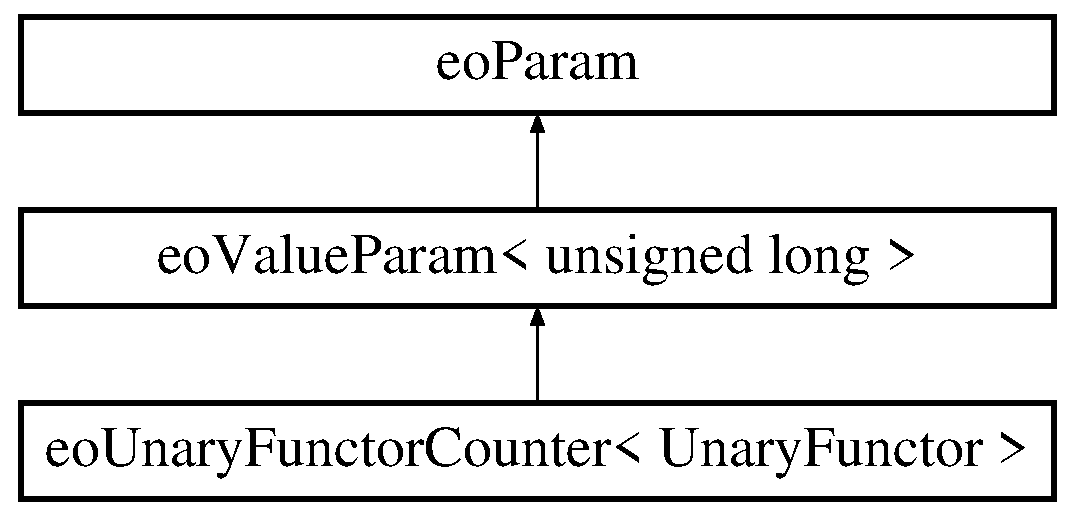
\includegraphics[height=3cm]{classeo_unary_functor_counter}
\end{center}
\end{figure}
\subsection*{Public Member Functions}
\begin{CompactItemize}
\item 
{\bf eo\-Unary\-Functor\-Counter} (Unary\-Functor \&\_\-func, std::string \_\-name=\char`\"{}uf\_\-counter\char`\"{})\label{classeo_unary_functor_counter_a0}

\item 
Unary\-Functor::result\_\-type {\bf operator()} (typename Unary\-Functor::first\_\-argument\_\-type \_\-arg1)
\begin{CompactList}\small\item\em Calls the embedded function and increments the counter. \item\end{CompactList}\end{CompactItemize}
\subsection*{Private Attributes}
\begin{CompactItemize}
\item 
Unary\-Functor \& {\bf func}\label{classeo_unary_functor_counter_r0}

\end{CompactItemize}


\subsection{Detailed Description}
\subsubsection*{template$<$class Unary\-Functor$>$ class eo\-Unary\-Functor\-Counter$<$ Unary\-Functor $>$}

Generic counter class that counts the number of times a unary function is used. 

Add a unary function through its ctor and use this class instead of it.

It is derived from {\bf eo\-Value\-Param}{\rm (p.\,\pageref{classeo_value_param})} so you can add it to a monitor.

Example: suppose you have an {\bf eo\-Eval\-Func}{\rm (p.\,\pageref{classeo_eval_func})} called myeval, to count the number of evaluations, just define:

eo\-Unary\-Functor\-Counter$<$void, Eo\-Type$>$ eval\-Counter(myeval);

and use eval\-Counter now instead of myeval. 



Definition at line 95 of file eo\-Counter.h.

\subsection{Member Function Documentation}
\index{eoUnaryFunctorCounter@{eo\-Unary\-Functor\-Counter}!operator()@{operator()}}
\index{operator()@{operator()}!eoUnaryFunctorCounter@{eo\-Unary\-Functor\-Counter}}
\subsubsection{\setlength{\rightskip}{0pt plus 5cm}template$<$class Unary\-Functor$>$ Unary\-Functor::result\_\-type {\bf eo\-Unary\-Functor\-Counter}$<$ Unary\-Functor $>$::operator() (typename Unary\-Functor::first\_\-argument\_\-type {\em \_\-arg1})\hspace{0.3cm}{\tt  [inline]}}\label{classeo_unary_functor_counter_a1}


Calls the embedded function and increments the counter. 

Note for MSVC users, if this code does not compile, you are quite likely trying to count a function that has a non-void return type. Don't look at us, look at the MSVC builders. Code like \char`\"{}return void;\char`\"{} is perfectly legal according to the ANSI standard, but the guys at Microsoft didn't get to implementing it yet.

We had two choices: assuming (and compiling ) code that returns void or code that returns non-void. Given that in {\bf EO}{\rm (p.\,\pageref{class_e_o})} most functors return void, it was chosen to support void.

But also please let me know if you have a compiler that defines \_\-MSC\_\-VER (lot's of windows compilers do), but is quite capable of compiling return void; type of code. We'll try to change the signature then.

You happy GNU (and other compiler) users will not have a problem with this. 

Definition at line 118 of file eo\-Counter.h.

References eo\-Value\-Param$<$ unsigned long $>$::value().

The documentation for this class was generated from the following file:\begin{CompactItemize}
\item 
eo\-Counter.h\end{CompactItemize}
